\documentclass[../preview.tex]{subfiles}
\begin{document} 
\begin{figure}
\centering
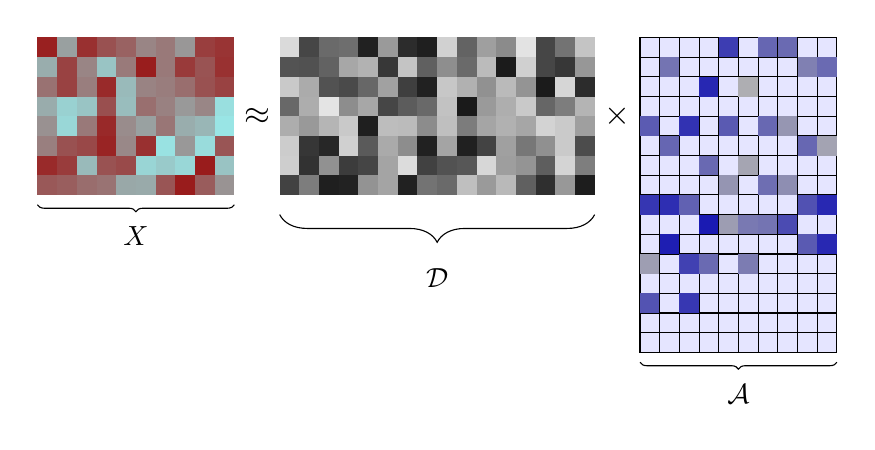
\begin{tikzpicture}
\def\N{8}
\def\S{10}
\def\D{16}
\def\sc{0.25}
\pgfmathtruncatemacro {\Na }{\N -1}
\pgfmathtruncatemacro {\Da }{\D -1}
\pgfmathtruncatemacro {\Sa }{\S -1}
%\draw (0, 0) grid (8, 4);
\matrix{
  {
      % Signal
      \begin{scope}[scale=\sc]
      \foreach \r in {0,...,\Na}{
          \foreach \c in {0,...,\Sa}{
              \pgfmathparse{0.8*rnd+0.1};
              \definecolor{MyColor}{rgb}{0.6,\pgfmathresult,\pgfmathresult}
              \fill[fill=MyColor] (\c, \r) rectangle +(1,1);
          }
      }
      \draw[decorate, decoration={brace, mirror}] (0, -.5) -- +(\S, 0) 
      node [black, midway, yshift=-0.4cm] {$X$};    
      \end{scope}
  }&
  {
      % = 
      \begin{scope}[scale=\sc]
      \path (0, 0) rectangle (1, 1);
      \node at (0.5, 4) {\large $\approx$};
      \end{scope}
  }&
  {
      % Dictionary
      \begin{scope}[scale=\sc]
      \foreach \r in {0,...,\Na}{
          \foreach \c in {0,...,\Da}{
              \pgfmathparse{0.8*rnd+0.1};
              \definecolor{MyColor}{rgb}{\pgfmathresult,\pgfmathresult,\pgfmathresult}
              \fill[fill=MyColor] (\c, \r) rectangle (\c+1,\r+1);
          }
      }
      \draw[decorate, decoration={brace, mirror, amplitude=10pt}] (0, -1) -- (\D, -1) 
      node [black, midway, yshift=-0.8cm] {$\mathcal{D}$};    
      \end{scope}
  } &
  {
      % multiplication
      \begin{scope}[scale=\sc]
      \path (0, 0) rectangle (1, 1);
      \node at (0.5, 4) {\large $\times$};
      \end{scope}
  } &
  {
      % Representation
      \begin{scope}[scale=\sc]
      \foreach \c in {0,...,\Sa}{
          \foreach \r in {0,...,\Da}{
              \pgfmathparse{0.8*rnd+0.1};
              \filldraw[fill=blue!10!] (\c, \r-\N) rectangle +(1,1);
          }
          \pgfmathrandominteger{\a}{0}{4}
          \foreach \r in {2, 4, 7, 11}{
              \pgfmathparse{0.6*rnd+0.1};
              \definecolor{MyColor}{rgb}{\pgfmathresult,\pgfmathresult, .7}
              \fill[fill=MyColor] (\c, \r+\a-\N) rectangle +(1,1);
          }
      }
      \draw[decorate, decoration={brace, mirror}] (0, -\N-.5) -- +(\S, 0) 
      node [black, midway, yshift=-0.4cm] {$\mathcal{A}$};    
      \end{scope}
  } 
  \\
};
\end{tikzpicture}

\end{figure}
\end{document}
